\documentclass[a4paper, 11pt, oneside]{article}

\usepackage[utf8]{inputenc}
\usepackage[T1]{fontenc}
\usepackage[french]{babel}
\usepackage{array}
\usepackage{shortvrb}
\usepackage{listings}
\usepackage[fleqn]{amsmath}
\usepackage{amsfonts}
\usepackage{fullpage}
\usepackage{enumerate}
\usepackage{graphicx}             % import, scale, and rotate graphics
\usepackage{subfigure}            % group figures
\usepackage{alltt}
\usepackage{url}
\usepackage{indentfirst}
\usepackage{eurosym}
\usepackage{listings}
\usepackage{color}
\usepackage[table,xcdraw,dvipsnames]{xcolor}

% Change le nom par défaut des listing
\renewcommand{\lstlistingname}{Extrait de Code}

% Change la police des titres pour convenir à votre seul lecteur
\usepackage{sectsty}
\allsectionsfont{\sffamily\mdseries\upshape}
% Idem pour la table des matière.
\usepackage[nottoc,notlof,notlot]{tocbibind}
\usepackage[titles,subfigure]{tocloft}
\renewcommand{\cftsecfont}{\rmfamily\mdseries\upshape}
\renewcommand{\cftsecpagefont}{\rmfamily\mdseries\upshape}

\definecolor{mygray}{rgb}{0.5,0.5,0.5}
\newcommand{\coms}[1]{\textcolor{MidnightBlue}{#1}}

\lstset{
    language=C, % Utilisation du langage C
    commentstyle={\color{MidnightBlue}}, % Couleur des commentaires
    frame=single, % Entoure le code d'un joli cadre
    rulecolor=\color{black}, % Couleur de la ligne qui forme le cadre
    stringstyle=\color{RawSienna}, % Couleur des chaines de caractères
    numbers=left, % Ajoute une numérotation des lignes à gauche
    numbersep=5pt, % Distance entre les numérots de lignes et le code
    numberstyle=\tiny\color{mygray}, % Couleur des numéros de lignes
    basicstyle=\tt\footnotesize,
    tabsize=3, % Largeur des tabulations par défaut
    keywordstyle=\tt\bf\footnotesize\color{Sepia}, % Style des mots-clés
    extendedchars=true,
    captionpos=b, % sets the caption-position to bottom
    texcl=true, % Commentaires sur une ligne interprétés en Latex
    showstringspaces=false, % Ne montre pas les espace dans les chaines de caractères
    escapeinside={(>}{<)}, % Permet de mettre du latex entre des <( et )>.
    inputencoding=utf8,
    literate=
  {á}{{\'a}}1 {é}{{\'e}}1 {í}{{\'i}}1 {ó}{{\'o}}1 {ú}{{\'u}}1
  {Á}{{\'A}}1 {É}{{\'E}}1 {Í}{{\'I}}1 {Ó}{{\'O}}1 {Ú}{{\'U}}1
  {à}{{\`a}}1 {è}{{\`e}}1 {ì}{{\`i}}1 {ò}{{\`o}}1 {ù}{{\`u}}1
  {À}{{\`A}}1 {È}{{\`E}}1 {Ì}{{\`I}}1 {Ò}{{\`O}}1 {Ù}{{\`U}}1
  {ä}{{\"a}}1 {ë}{{\"e}}1 {ï}{{\"i}}1 {ö}{{\"o}}1 {ü}{{\"u}}1
  {Ä}{{\"A}}1 {Ë}{{\"E}}1 {Ï}{{\"I}}1 {Ö}{{\"O}}1 {Ü}{{\"U}}1
  {â}{{\^a}}1 {ê}{{\^e}}1 {î}{{\^i}}1 {ô}{{\^o}}1 {û}{{\^u}}1
  {Â}{{\^A}}1 {Ê}{{\^E}}1 {Î}{{\^I}}1 {Ô}{{\^O}}1 {Û}{{\^U}}1
  {œ}{{\oe}}1 {Œ}{{\OE}}1 {æ}{{\ae}}1 {Æ}{{\AE}}1 {ß}{{\ss}}1
  {ű}{{\H{u}}}1 {Ű}{{\H{U}}}1 {ő}{{\H{o}}}1 {Ő}{{\H{O}}}1
  {ç}{{\c c}}1 {Ç}{{\c C}}1 {ø}{{\o}}1 {å}{{\r a}}1 {Å}{{\r A}}1
  {€}{{\euro}}1 {£}{{\pounds}}1 {«}{{\guillemotleft}}1
  {»}{{\guillemotright}}1 {ñ}{{\~n}}1 {Ñ}{{\~N}}1 {¿}{{?`}}1
}
\newcommand{\tablemat}{~}

%%%%%%%%%%%%%%%%% TITRE %%%%%%%%%%%%%%%%
% Complétez et décommentez les définitions de macros suivantes :
\newcommand{\intitule}{Récursivité et Élimination de la Récursivité}
\newcommand{\Prenom}{Maxime}
\newcommand{\Nom}{Deravet}
\newcommand{\matricule}{s202214}
% Décommentez ceci si vous voulez une table des matières :
\renewcommand{\tablemat}{\tableofcontents}

%%%%%%%% ZONE PROTÉGÉE : MODIFIEZ UNE DES DIX PROCHAINES %%%%%%%%
%%%%%%%%            LIGNES POUR PERDRE 2 PTS.            %%%%%%%%
\title{INFO0947: \intitule}
\author{\textsc{\Prenom}~\textsc{\Nom}, \matricule}
\date{}

\begin{document}
\maketitle
\newpage
\tablemat
\newpage
%%%%%%%%%%%%%%%%%%%% FIN DE LA ZONE PROTÉGÉE %%%%%%%%%%%%%%%%%%%%

%%%%%%%%%%%%%%%% RAPPORT %%%%%%%%%%%%%%%
% Complétez les sections ci-dessous

\section{Formulation Récursive}\label{formulation}
%%%%%%%%%%%%%%%%%%%%%%%%%%%%%%%%
%
% Fournissez et discutez ici la formulation récursive du problème
%

$\sum\limits_{i=0}^{n-1}    a_{i} \times 16^{ n-1}$
\\
\\
a étant le nombre retourné par convert(),\\ i le rang dans la chaine de caractères,\\ et n la taille de la chaine de caractères soustrait du rang



\section{Spécification}\label{specification}
%%%%%%%%%%%%%%%%%%%%%%%%%
%
% Fournissez et discutez ici la spécification formelle de la fonction
% hexa_dec_rec()
%


\begin{flushleft}
    \bf
    Préconditions
\end{flushleft}

La chaîne de caractères hexa doit être composée de caractères repris dans l'hexadécimal, autrement dit des chiffres compris entre 0 et 9 ou des lettres de A à F.
\\
n doit être égal à la taille de hexa
\\


\begin{flushleft}
    \bf
Postconditions
\end{flushleft}

La fonction hexa\_dec\_rec() renvoie l'équivalent du nombre hexadécimal entré en base 10






\section{Construction Récursive}\label{recur}
%%%%%%%%%%%%%%%%%%%%%%%%%%%%%%%%%
%
% Fournissez et discutez ici la construction formelle (avec les assertions
% intermédiaires) de la fonction hexa_dec_rec()
%


\begin{flushleft}
    \bf
    Programmation défensive :
\end{flushleft}

On vérifie que le tableau n'a pas de valeur négative, et que les caractères rentrés sont bien hexadécimaux.

\begin{lstlisting}[caption={Programmation défensive}]
/**
* Précondition : - Hexa doit être une chaine de caractères composée de chiffres
*compris entre 0 et 9 ou des lettres comprises entre A et F
*                - n doit être égal à la taille de la chaine hexa
* Postcondition : retourne le nombre hexadécimal entré en base 10
*
*/
unsigned int hexa_dec_rec(char *hexa, int n)

\end{lstlisting}


%%%%%


\begin{flushleft}
    \bf
    Cas récursif :
\end{flushleft}

Il n'y a qu'un cas récursif, si n >0\\
(L'assertion vérifie la valeur maximale d'un int, car la fonction unsigned int convert renvoie -1)

\begin{lstlisting}[caption={Cas récursif}]
  if (n >0){
    assert(convert(hexa[n-1]) != 4294967295);
    nombre = convert(hexa[n-1]);
    return nombre + 16 * hexa_dec_rec(hexa, n-1);
  }

\end{lstlisting}


%%%%
\begin{flushleft}
    \bf
    Cas de base :
\end{flushleft}

Simplement si n == 0, alors la fonction renvoie 0

\begin{lstlisting}[caption={Cas de base}]
else
  return 0;

\end{lstlisting}

%%%


\begin{flushleft}
    \bf
    Code complet :
\end{flushleft}

Le unsigned int nombre est juste là pour rendre le code plus lisible, mais n'a pas d'autres utilités.

\begin{lstlisting}[caption={Cas de base}]
/**
* Précondition : - Hexa doit être une chaine de caractères composée de chiffres
*compris entre 0 et 9 ou des lettres comprises entre A et F
*                - n doit être égal à la taille de la chaine hexa
* Postcondition : retourne le nombre hexadécimal entré en base 10
*
*/
unsigned int hexa_dec_rec(char *hexa, int n){
   assert(n>-1);


  unsigned int nombre;


  if (n >0){
    assert(convert(hexa[n-1]) != 4294967295);
    nombre = convert(hexa[n-1]);
    return nombre + 16 * hexa_dec_rec(hexa, n-1);
  }

else
  return 0;

\end{lstlisting}





\section{Traces d'Exécution}\label{traces}
%%%%%%%%%%%%%%%%%%%%%%%%%%%%%
%
% Fournissez et discutez ici les traces d'exécution de la fonction romain_rec()
% pour les exemples donnés dans l'énoncé
%

\newpage
\section{Complexité}\label{complexite}
%%%%%%%%%%%%%%%%%%%%%
%
% Fournissez et discutez ici la complexité théorique de la fonction
%  hexa_dec_rec()
%
Le corps de la fonction, avec découpe en régions, est le suivant :

\vfill
\begin{center} 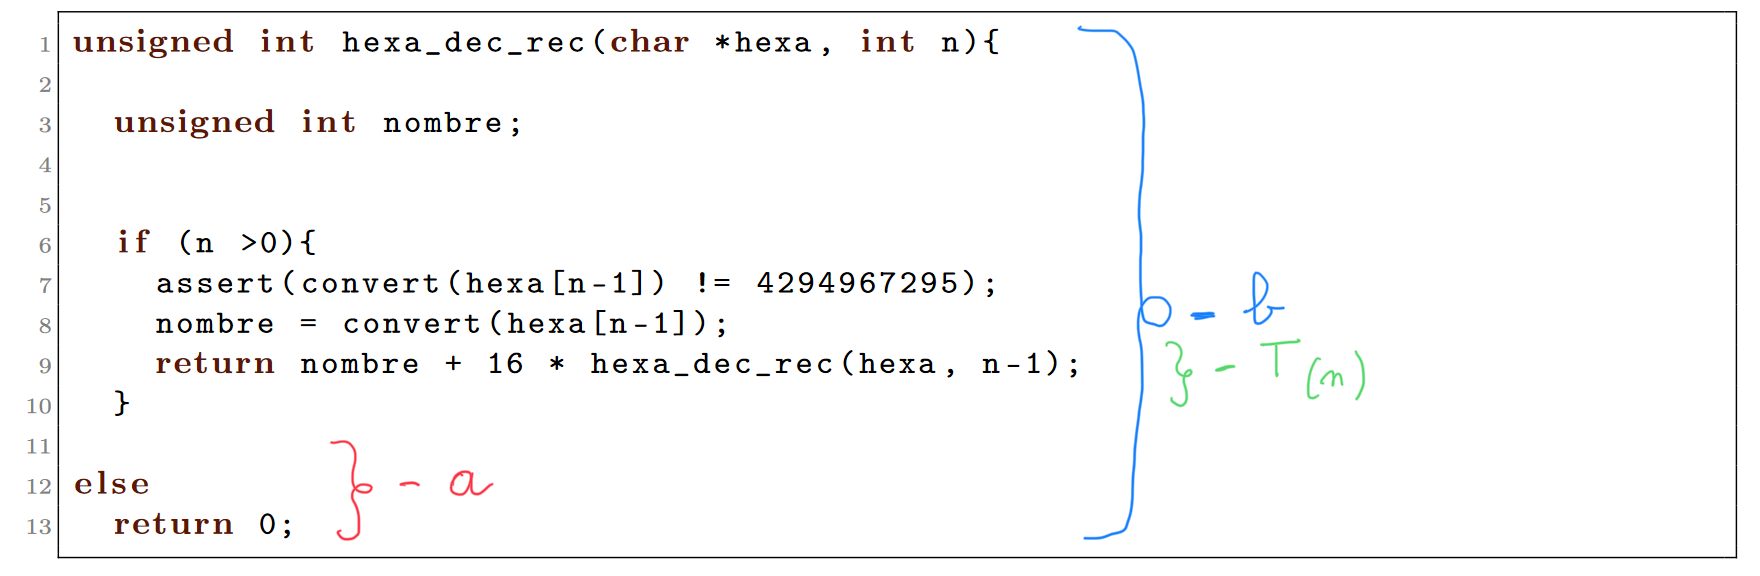
\includegraphics[scale=0.25]{image.png} \end{center}
\vfill

On peut faire une telle découpe. En fait, on considère qu’ils vont impliquer autant d’opérations élémentaires :b. Par contre, le temps pris par l’appel récursif est bienT(n).On obtient alors le système suivant :


\begin{equation*}
T(n) =
\begin{cases}
a & \text{si } n = 0,\\
b + T(n) & \text{sinon } \\

\end{cases}
\end{equation*}
\\

Il y a bien une addition entre b et T(n) parce qu’il faut d’abord faire b opérations,puis, il faut exécuter 1 appel récursif. Résolvons l’équation de récurrence par application de la méthode de proche en proche :


\begin{align}
T(n) & = b + T(n) \\
& = 2 \times b + 2 \times T(n) \\
& = 3 \times b + 3 \times T(n) \\
& = ... \\
& = k \times b + k \times T(n) \\
\end{align}
\\
On sait que : \\
 T(1) =b+T(0) =b+a \\

 Essayons de faire apparaitre T(1) à la place de T(n) :\\
 T(1) = b + T(0) = b + a \\
 n = 1 \\
 n = k \\
 \newpage
 Il vient alors:

\begin{align}
T(n) & = k \times b + k \times T(n)\\
& = b \times n + b + a  \in O(n)\\
\end{align}
Nous avons donc une complexité linéaire












\section{Dérécursification}\label{derecur}
%%%%%%%%%%%%%%%%%%%%%%%%%%%%
%
% Fournissez et discutez ici la dérécursification de la fonction hexa_dec_rec()
% Attention, il n'est pas question ici de fournir un algorithme itératif mais
% bien d'éliminer la récursivité comme cela a été vu au cours.
% La solution doit être proposée en utilisant le pseudo-code vu au cours (et
% dans les GameCodes du Chapitre 9).
%

\end{document}
